%Correct the file name.
%X: book number
%Y: part number
%ZZZ: page number in three digits. So page 3 would be 003.

\documentclass[11pt]{amsbook}

\usepackage{../HBSuerDemir}	% ------------------------
\usepackage{amssymb}

\begin{document}

% ++++++++++++++++++++++++++++++++++++++
\hPage{b1p2/351}
% ++++++++++++++++++++++++++++++++++++++

Let 
$$ \Delta x_i=x_i-x_{i-1}, \hspace{1cm} t_i \in
\Big( x_i, x_{i-1}  \Big), \hspace{1cm} i=1,......, n
$$
and consider the sum 
$$ I_n= \sum_{i=1}^{n} \hspace{.3cm} f(t_i)\Delta x_i $$
called the \underline{RIEMANN Sum} (\underline{DARBOUX Sum})\\

Let $m_i=min \hspace{.15cm}f(x),\hspace{.2cm} M_i= max \hspace{.15cm}f(x)\hspace{.2cm} on \hspace{.2cm}\Big( x_{i-1}, x_i \Big)$ 
\hspace{.2cm}so that\newline we have 
$$ 
m_i \leq f(x) \leq M_i \hspace{1cm}for\hspace{1cm}x \in \Big( x_{i-1}, x_i \Big)
$$

and 
$$
\sum_{i=1}^{n} \hspace{.2cm} m_i\Delta x_i \hspace{.1cm}\leq\hspace{.1cm} I_n\hspace{.1cm} \leq \hspace{.1cm} \sum_{i=1}^{n} \hspace{.2cm} M_i\Delta x_i
$$\\

where we call the left hand  and right hand summations \emph{the lover sum} and \emph{the upper sum} respectively for the given partition P, that we denote by $L_n$ and $U_n$: 
$$
L_n \leq I_n \leq U_n
$$\\
If $L_n$ and $U_n$ have the same limit for all partitions as $n\rightarrow\infty$ and $m\geq x \hspace{.3cm}\Delta x_i \rightarrow 0 $, then $I_n$ tends  to this common limit, and this common limit is denoted by\\
\paragraph{\hspace{1cm}$\int\limits_a^b \hspace{.1cm} f(x)dx$ \hspace{.5cm} (Read: integral from a to b of f(x)dx)\newline}

\paragraph{As to existence of limit we have the following theorem whose proof is given in Advanced Calculus:}


\paragraph{\underline{Theorem}. $f(x) \in C(a,b) \implies \int\limits_a^b \hspace{.1cm} f(x)dx$ exists.}


\paragraph{This definite integral is the \emph{RIEMANN integral} of $f(x)$ over the closed interval $(a, b)$, and $f(x)$ is said to be \emph{RIEMANN integrable} function, where a and b are the \emph{lover limit} and \emph{upper limit} of the integral, respectively.}

\paragraph{\underline{Example 1}. Evaluate \hspace{.2cm}$\int\limits_a^b \hspace{.1cm} dx$}



\end{document}  

%==== templates ====

%==== environments ====

%\begin{figure}[htb]
%	\centering
%	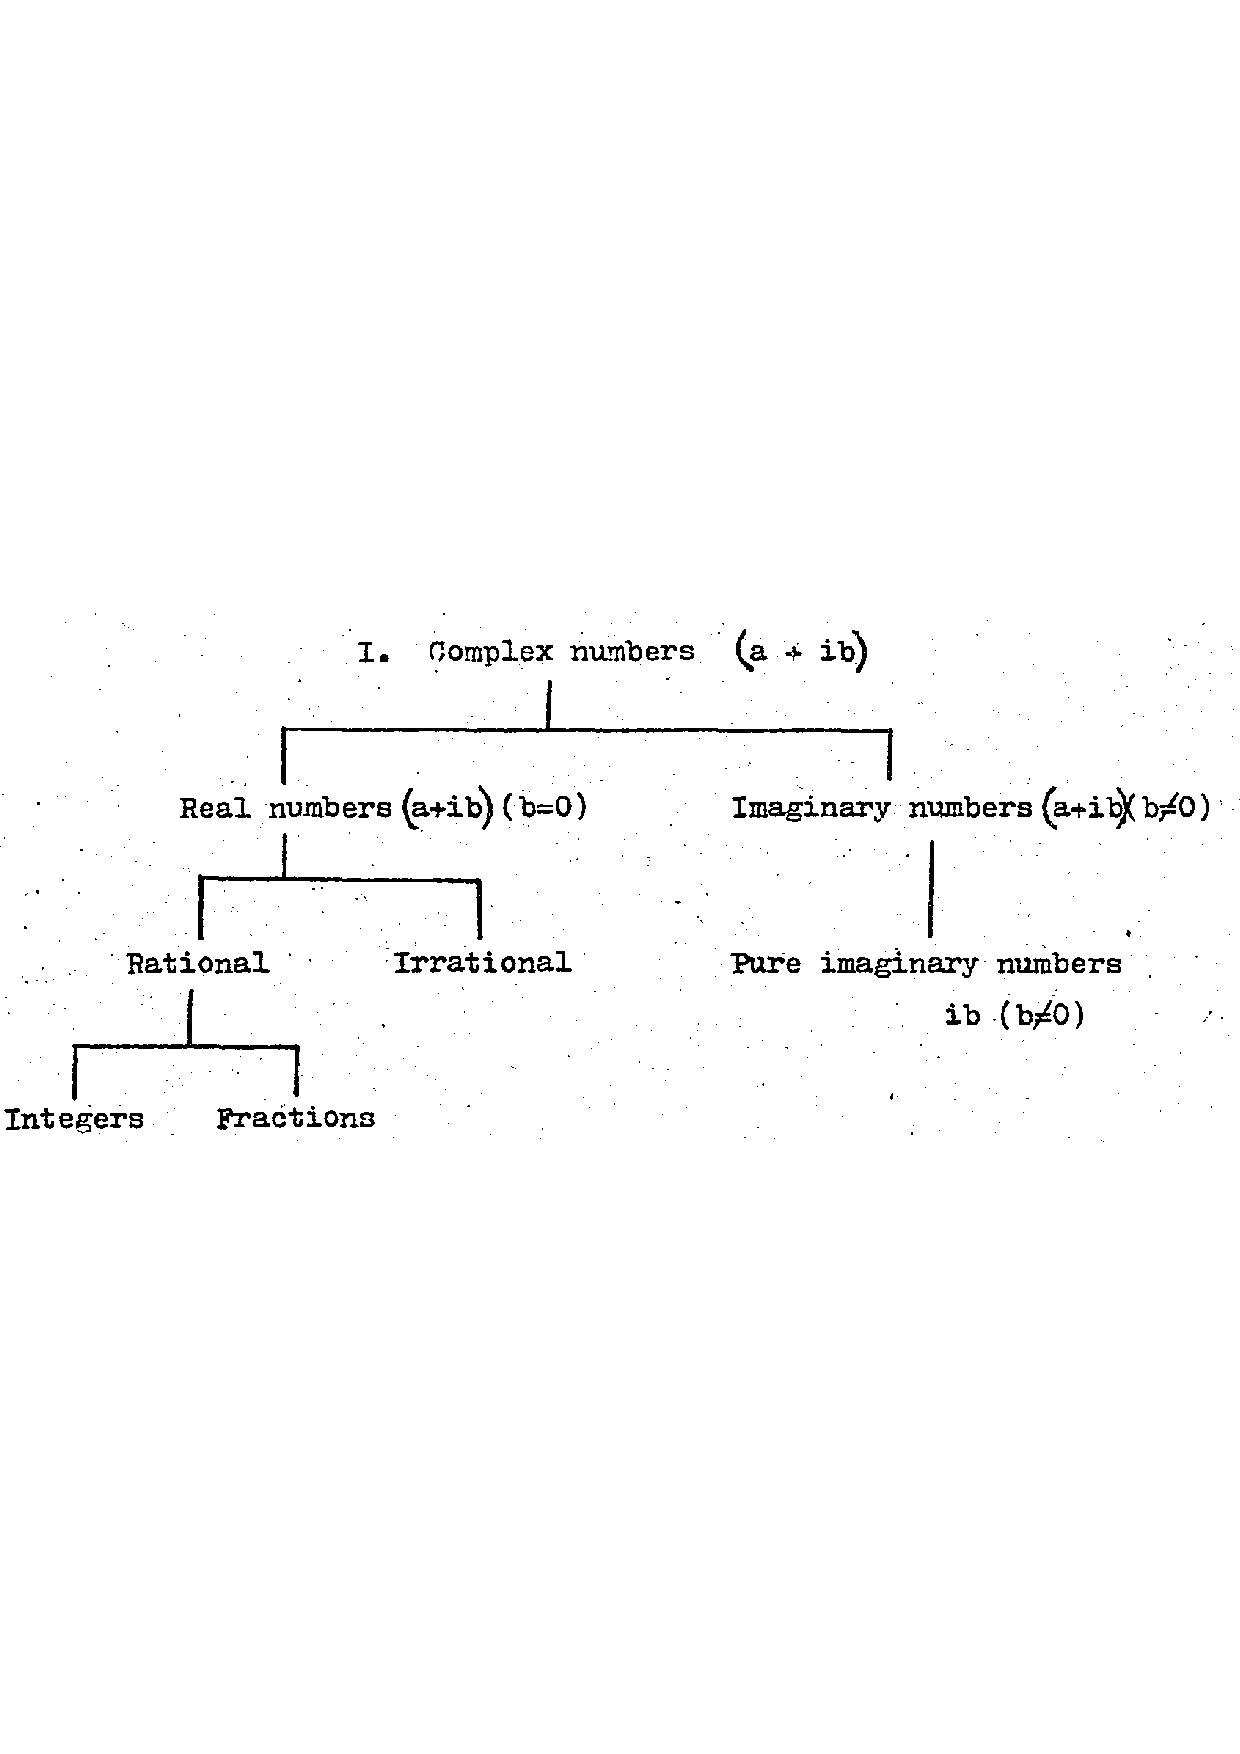
\includegraphics[width=0.9\textwidth]{images/SD-1-1p15A}
%	\caption{Classification of complex numbers}
%	\label{fig:classificationOfComplexNumbersA}
%\end{figure}

%\begin{center}
%\begin{tabular}{cc}
%\end{tabular}
%\end{center}

%\begin{exmp}
%\begin{hSolution}
%\end{hSolution}
%\end{exmp}

%\begin{hEnumerateAlpha}
%\end{hEnumerateAlpha}

%\begin{hEnumerateRoman}
%\end{hEnumerateRoman}

%$
%\begin{bmatrix}
%\end{bmatrix}
%$

%\frac{aaaa}{bbb}
%\frac{a_{n}}{b_{n}}
%\left( aaaa \right)
%\Longrightarrow

%\begin{multicols}{2}
%	bb
%\columnbreak
%	aa
%\end{multicols}
